\documentclass{article}
\usepackage{stmaryrd}
\usepackage{graphicx}

\title{Report, Kinetic project}
\author{Dorian Geraldes Pereira, Axel Demuth}
\date{March 2024}

\begin{document}
\maketitle
\tableofcontents
\newpage
\section{Objectives}
the objective of the project is to process files in IFC format containing building meshes that are not hermetic in an algorithms repairing
geometric error in a kinetic data structures
\section{Tools}
\subsection{CGAL}
CGAL is a comprehensive package for geometry algorithms, providing various data structures and algorithms for working on polygons, surfaces, mesh generation, and more.
It offers a wide range of functionalities for geometric processing and analysis in various fields such as computer graphics, computational geometry, and geometric modeling.
\subsection{Kinetic}

Kinetic algorithms is a package from CGAL that allows working on meshes with some holes in them. When applied to the mesh, the Kinetic algorithms will 'extend' some surfaces to fill the mesh and make it watertight. 
Here's what the algorithm is capable of:


\begin{figure}[h]
    
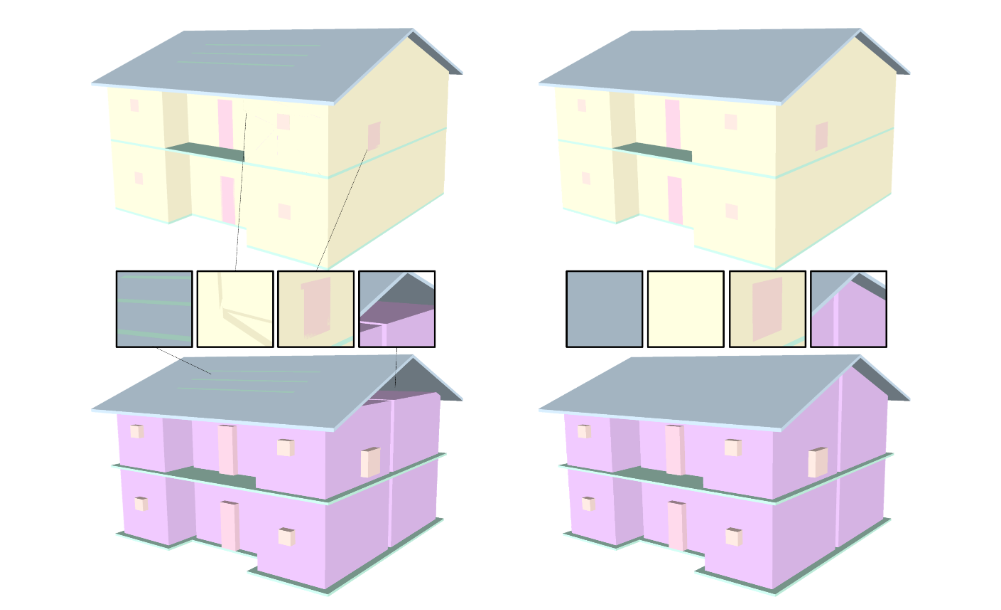
\includegraphics[scale =   0.3 ]{../../images/example_algorithm.png}

\end{figure}

\newpage
We intend to work on this project in the coming months and will continuously update our progress as outlined in the following roadmap.
\begin{figure}[h]
    
    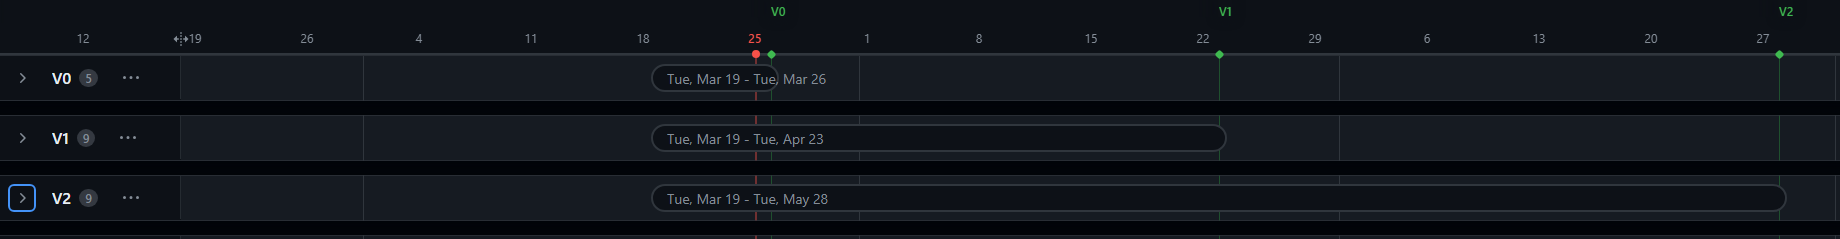
\includegraphics[scale =   0.3 ]{../../images/roadmap.png}
    
    \end{figure}
    
\nocite{*}
\bibliographystyle{plain}
\bibliography{../../bibliography/v0/report_bib}
\end{document}